\chapter{Methodik}

Wie schon im vorherigen Kapitel beschrieben müssen additiv gefertigte Bauteile 
nachbearbeitet werden, bevor sie eingesetzt werden können. In Abbildung~\ref{fig:post-pro}
ist ein additiv gefertigtes Metallbauteil vor und nach der Nachbearbeitung dargestellt.
In der Nachbearbeitung wurden die Stützstrukturen entfernt und die Güte der Oberfläche 
verbessert. 
Der Nachbearbeitungsschritt wird nicht nur zur optischen Verbesserung verwendet, sondern 
auch zur Verbesserung der physikalischen und mechanischen Eigenschaften. 
Zum Beispiel kann durch eine Laserbearbeitung der Härtegrad des Bauteils erhöht 
werden~\cite{Mahmood.2022}.

\begin{figure}[H]
    \centering
    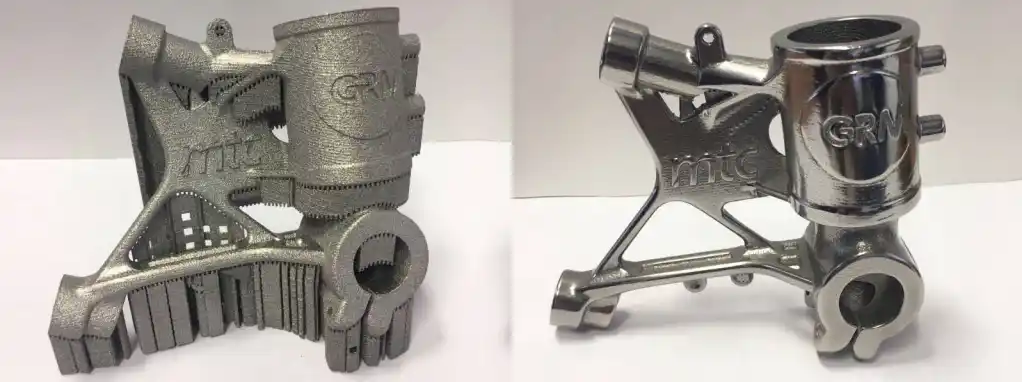
\includegraphics[width=0.8\textwidth]{images/post-processing.PNG}
    \caption{Ein additiv gefertigtes Metallbauteil vor und nach der Nachbearbeitung
    ~\cite{unionfab.22.08.2023}}
    \label{fig:post-pro}
\end{figure}

Um eine korrekte Nachbearbeitung gewährleisten zu können, muss das additiv 
gefertigte Bauteil fixiert werden, so wird verhindert das sich das Bauteil während der 
Nachbearbeitung räumlich verschiebt. Durch eine Verschiebung kann das Bauteil oder das, für
die Nachbearbeitung verwendete Werkzeug, beschädigt werden. Bei einer händischen 
Nachbearbeitung kann sogar die Gesundheit der Arbeitskraft in Mitleidenschaft gezogen werden.
Eine Option das Bauteil für die Nachbearbeitung zu fixieren, ist ein Schraubstock. 
Hier wird das Bauteil zwischen zwei Backen eingespannt und so verhindert, dass sich das
Bauteil während des Nachbearbeitungsprozesses verschiebt. Durch das Einspannen wirkt eine 
Kraft auf das Bauteil. Diese Spannkraft kann sich auf die Form des Bauteils auswirken, für 
die weitere Verwendung des Bauteils ist es nötig, dass das Bauteil genau die geforderte 
Geometrie, also die des CAD-Designs, hat. Falls dies nicht der Fall ist, kann das Bauteil
unter Umständen nicht mehr wie vorgesehen eingesetzt werden.

Für die Beurteilung, ob ein Bauteil noch eingesetzt werden kann, ist es nötig die 
Deformation die auf das Objekt gewirkt hat zu erkennen. Durch die Analyse der Spannkraft 
und Deformation eines Bauteils kann anschließend zu der Nachbearbeitung ermittelt werden, 
ob sich das Bauteil nachhaltig deformiert hat.

\section{Verfahren zur optische Spannkraftdeformationserkennung}

Um die Deformation des Bauteils erfassen zu können wird das 3D-Objekt benötigt, 
dass als Grundlage für die AF dient. Zusätzlich werden optische Daten des Bauteils 
im deformiertem Zustand benötigt. Mit diesen beiden Daten kann der Unterschied 
ermittelt und ausgegeben werden.
Um auch minimale Deformationen erkennen zu können, müssen die Daten des 
eingespannten Bauteils hinreichend genau sein. Aus diesem Grund wird ein Laserscanner zur 
Datenerfassung eingesetzt.
Wie schon beschrieben ist der Messbereich eines Laserscanners begrenzt. Da das 
Verfahren nicht auf eine Bauteilgröße beschränkt sein soll, müssen mehrere Scans als 
Eingabe akzeptiert werden.

\section{Vorgehen}

Das Verfahren, um eine Deformation in einem eingespannten additiv gefertigten
Bauteil, zu erkennen, soll folgende Schritte umfassen:
\begin{itemize}
    \item \textbf{Aufnahme der Scandaten}\\
        Zu Beginn sollen die Daten, aus denen die Deformation erkannt werden soll, 
        aufgenommen werden. Hierfür soll ein Laserscanner verwendet werden, durch diesen wird 
        das Bauteil im eingespannten Zustand gescannt. Zusätzlich soll die 
        Verschiebung im Schraubstock durch einen Verschiebungsmesser gemessen werden.
        Die Spannkraft, die auf das Bauteil wirkt, wird durch zwei Kraftmesser im 
        Schraubstock gemessen.
    \item \textbf{Digitalisierung des Bauteils:}\\
        In diesem Schritt sollen Messfehler und Ausreißer
        in den Scandaten entfernt werden. Anschließend werden die dreidimensionalen 
        Eingangsdaten in eine zweidimensionale Ansicht umgewandelt.
        Nach diesem Schritt sollen für jedes Bauteil mehrere Datensätze als 
        zweidimensionale schwarz weiß Bilder vorliegen.
    \item \textbf{Stitching Methodik}\\
        Die vorliegenden Bilder sollen nun zu einem einzelnen Bild zusammengefügt werden.
        Hierfür werden Gemeinsamkeiten in den sich 
        überlappenden Bildern gesucht und eine Transformation ermittelt,
        die auf eines von zwei Bildern angewendet werden kann, um sie zusammenzufügen.
    \item \textbf{Deformationserkennung}\\
        Wenn ein Bild für ein eingespanntes Bauteil vorliegt, sollen verschiedene 
        Zustände des Bauteils verglichen werden. Deformationen können erkannt werden, in dem 
        die Länge und Breite des Bauteils verglichen wird, zusätzlich wird der 
        Abstand zwischen den Rändern des Bauteils berechnet. Es sollen verschiedene
        Spannungszustände verglichen werden können. Ein Vergleich mit dem initialen 
        CAD-Design ist auch möglich, hier sollen auch Fehler erkannt werden, die im 
        Fertigungsprozess entstehen. Der Unterschied zwischen Bauteilzuständen
        soll visuell ausgegeben werden und als Bild gespeichert werden.
        
\end{itemize}
























